\documentclass{standalone}

\usepackage{tikz}
\usetikzlibrary{mindmap}

\pgfdeclarelayer{background}

\begin{document}

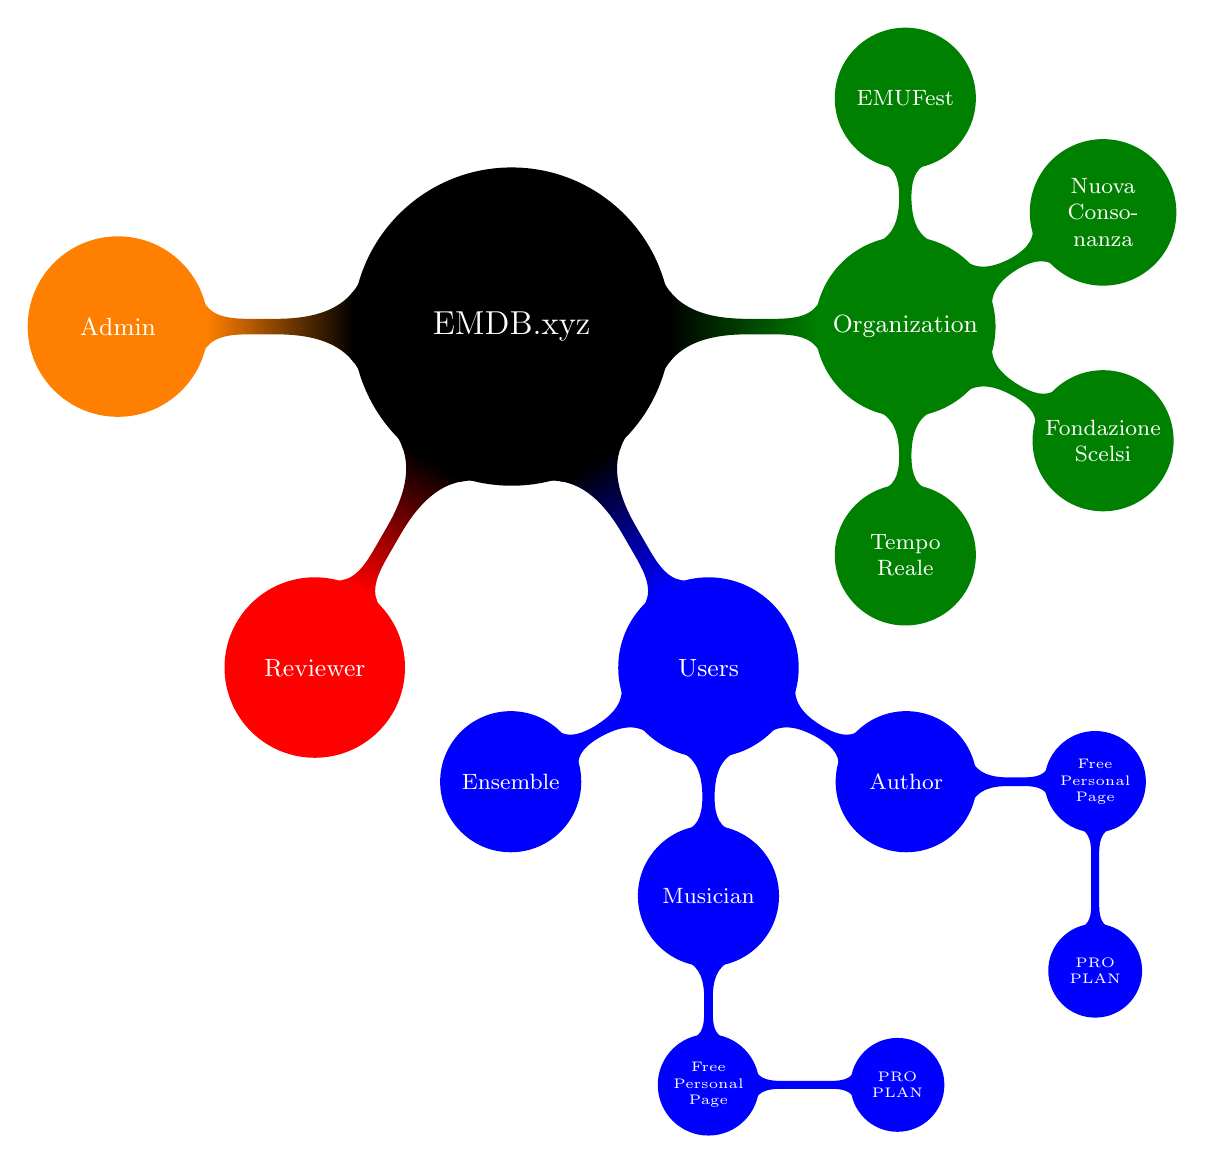
\begin{tikzpicture}
  \path[mindmap,concept color=black,text=white]
    node[concept] {EMDB.xyz}
	[clockwise from=0]
    child[concept color=green!50!black] {
      node[concept] {Organization}
      [clockwise from=90]
      child { node[concept] (emu) {EMUFest} }
      child { node[concept] (nc)  {Nuova Consonanza} }
      child { node[concept] (fs)  {Fondazione Scelsi} }
      child { node[concept] (tr)  {Tempo Reale} }
    }
	child[concept color=blue] {
		node[concept] {Users}
		[clockwise from=-30]
		child { node[concept] (aut) {Author}
		[clockwise from=0]
			child { node[concept] {Free Personal Page}}
		[clockwise from=-90]
			child { node[concept] {PRO PLAN}}}
		child { node[concept] {Musician}
		[clockwise from=-90]
			child { node[concept] {Free Personal Page}}
		[clockwise from=0]
		child { node[concept] {PRO PLAN}}}
		child { node[concept] {Ensemble}}
    }
    child[concept color=red] { node[concept] {Reviewer} }
    child[concept color=orange] { node[concept] {Admin} };

\end{tikzpicture}

\end{document}
